\documentclass[12pt]{article}
\usepackage{times}
\usepackage[english]{babel}
\usepackage[utf8x]{inputenc}
\usepackage[colorinlistoftodos]{todonotes}
\usepackage[margin=1in]{geometry}
\usepackage{graphicx}
\usepackage{epstopdf}
\usepackage{cite}
\usepackage{listings}
\usepackage{dtklogos}
\usepackage{wrapfig}
\usepackage{subfigure}
\usepackage{amsmath}
\usepackage{amsthm}
\usepackage{amssymb}
\usepackage{amscd}
\usepackage{caption}
\usepackage{etoolbox}
\usepackage{fancyhdr}
\usepackage{stackengine}
\usepackage[export]{adjustbox}
\usepackage{url}
\patchcmd{\thebibliography}{\section*{\refname}}{}{}{}
\usepackage[document]{ragged2e}    %This causes text to left align
\usepackage[colorlinks=true, linkcolor=black,citecolor=black,urlcolor=blue]{hyperref}
\bibliographystyle{IEEEtran}
\DeclareGraphicsRule{.tif}{png}{.png}{`convert #1 `dirname #1`/`basename #1 .tif`.png}

\title{MCHE 358: Report 6}

\begin{document}
\lefthyphenmin3
\righthyphenmin4
% \pretolerance=2000
% \tolerance=500 
% \emergencystretch=10pt
%\raggedright     %Stops LaTeX from automatically hyphenating the right margin to fit better
%Combine this with \usepackage[document]{ragged2e} to get a text align left similar to natural MS Word
%-------------------------------------------------------------
%Header
%-------------------------------------------------------------
\fancyhf{}  
  \renewcommand{\headrulewidth}{0pt}
  \fancypagestyle{plain}{
    \fancyhead[R]{\thepage}} 
    \pagestyle{plain}
    
\captionsetup[table]{labelsep=space}

\begin{flushleft}
\hrulefill\\\hrule height 1pt
\vspace{5pt}
\textbf{DATE: } \hspace{20pt} \today
\bigskip\\
\textbf{TO: } \hspace{33pt} Sally Anne McInerny, Ph.D.\\ \hspace{60pt} Department of Mechanical Engineering
\bigskip\\
\textbf{FROM: } \hspace{13pt} Matthew J. Begneaud
\bigskip\\
\textbf{COPY: } \hspace{18pt} John Guillory, Ph.D.\\ \hspace{60pt} Department of Mechanical Engineering
\bigskip\\
\textbf{SUBJECT:} \hspace{2pt} Honda EM5000SX Engine-Generator System Performance
\vspace{-10pt}
\end{flushleft}
\hrulefill \hrule height 1pt

%-------------------------------------------------------------
%Start of Paper
%-------------------------------------------------------------

\section*{\fontsize{12}{12}\selectfont INTRODUCTION}
This memorandum conveys the findings of an experiment conducted to observe the performance of a Honda EM5000SX engine-generator system. The objectives of this experiment are to:

\begin{itemize}

\item Take various measurements during the experiment in order to calculate the Specific Fuel Consumption (SFC) and thermal efficiency as functions of power supplied by the generator.
\item Determine regression models for SFC and thermal efficiency which best fits the data recorded from the experiment.

\end{itemize}


It is useful for one to know how much fuel is consumed by an engine-generator system, as well as its thermal efficiency, based on what electrical power it will be supplying. It is expected that the engine's SFC and thermal efficiency should be similar to that of other small engine-generator systems, as seen in Figure 1 and Figure 2 \cite{Silva}. 
\bigskip

The equations used to calculate the SFC and thermal efficiency of the engine-generator using the data recorded in the experiment can be seen in Equation (1) and Equation (2) respectively, where $P$ is the electric power generated by the system. By observation of Equation (1) and Equation (2), it is expected that a power law regression should fit the experiment data well for both SFC and thermal efficiency. The fuel used in the experiment is approximately equivalent to liquid octane, $C_{8}H_{18}$.
\bigskip
\bigskip


\begin{equation}
SFC = \frac{\dot{m}}{P}
\end{equation}

\begin{equation}
\eta_{th} = \frac{P}{\dot{m}LHV_{C_{8}H_{18}}}
\end{equation}


\newpage


% Figure 1 - Reference SFC curve
\begin{figure}[h!] %  figure placement: here, top, bottom, or page
   \centering
   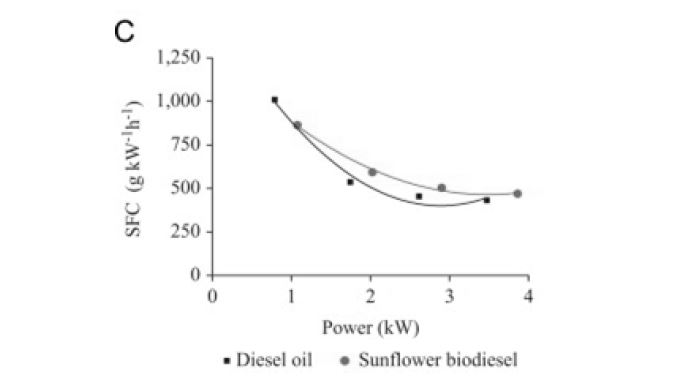
\includegraphics[width=6in]{SFC_reference.JPG} 
   \caption{SFC of Small Engine-Generator Systems}
   \label{fig:example}
\end{figure}

% Figure 2 - Reference thermal efficiency curve
\begin{figure}[h!] %  figure placement: here, top, bottom, or page
   \centering
   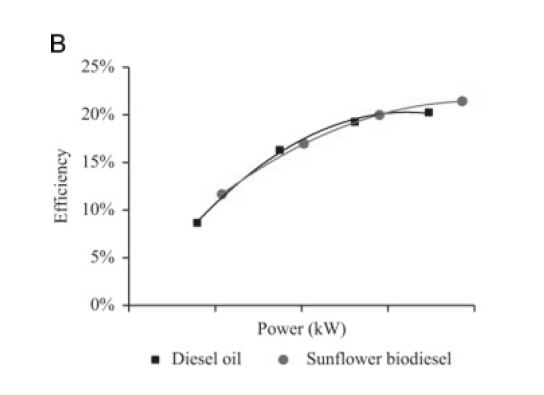
\includegraphics[width=5in]{thermal_efficiency_reference.jpg} 
   \caption{Thermal Efficiency of Small Engine-Generator Systems}
   \label{fig:example}
\end{figure}


\newpage


% Figure 3 - System diagram
\begin{figure}[h!] %  figure placement: here, top, bottom, or page
   \centering
   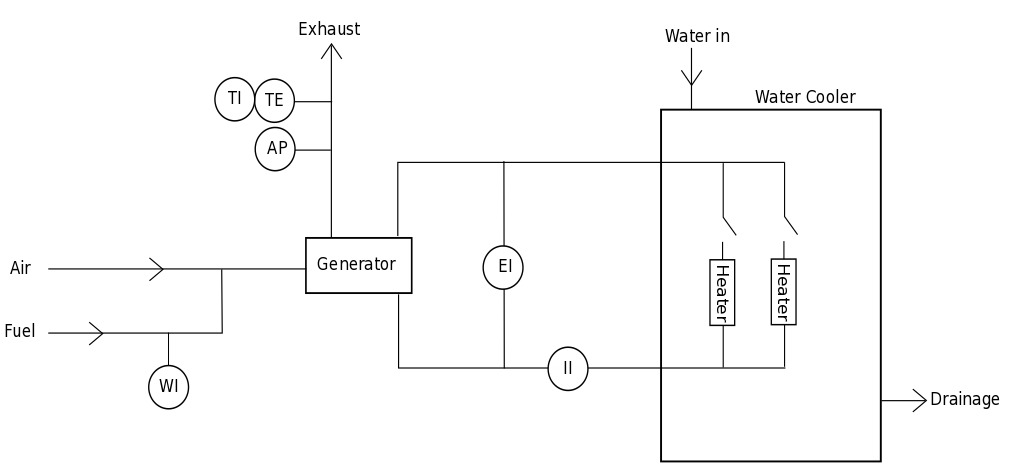
\includegraphics[width=\linewidth]{system_diagram.png} 
   \caption{Experiment System Diagram}
   \label{fig:example}
\end{figure}

\section*{\fontsize{12}{12}\selectfont PROCEDURE}
The experiment system diagram is shown in Figure 3. The system consists of an engine-generator system running on 87-octane fuel without ethanol, connected to a variable load in the form of resistance heaters. These heaters are contained inside a water tank to deposit the thermal energy into water moving through the tank. The weight of the fuel in the fuel tank is measured before it leaves to enter the combustion chamber. The exhaust temperature and carbon monoxide and oxygen content of the exhaust are measured at the exhaust outlet of the engine.
\bigskip

Experiment procedures were as follows. The engine was started and connected to a load. Once the engine began to run at steady state, the weight of the fuel was measured. After three minutes, the fuel weight was then measured again. The voltage across the generator output was also measured during each run of the experiment as well as the current through the circuit to determine the power provided by the generator. The load was changed for each run of the experiment.

\section*{\fontsize{12}{12}\selectfont DATA PRESENTATION \& ANALYSIS}
The data was used to calculate the Specific Fuel Consumption (SFC) and thermal efficiency of the engine for each run of the experiment, as well as the power supplied to the resistance heaters by the generator. The SFC is plotted in Figure 4 as a function of power generated with a power-law regression fitted to the data. The regression can be seen in Equation (3), and the correlation coefficient is calculated to be $r_{SFC}=0.99$. The thermal efficiency is also plotted as a function of power generated, and can be seen in in Figure 5 along with a power-law regression fitted to the data. The regression for thermal efficiency can be seen in Equation (4), and the correlation coefficient is calculated to be $r_{th} = 0.99$.
\bigskip

% Figure 4 - SFC vs Power
\begin{figure}[t!] %  figure placement: here, top, bottom, or page
   \centering
   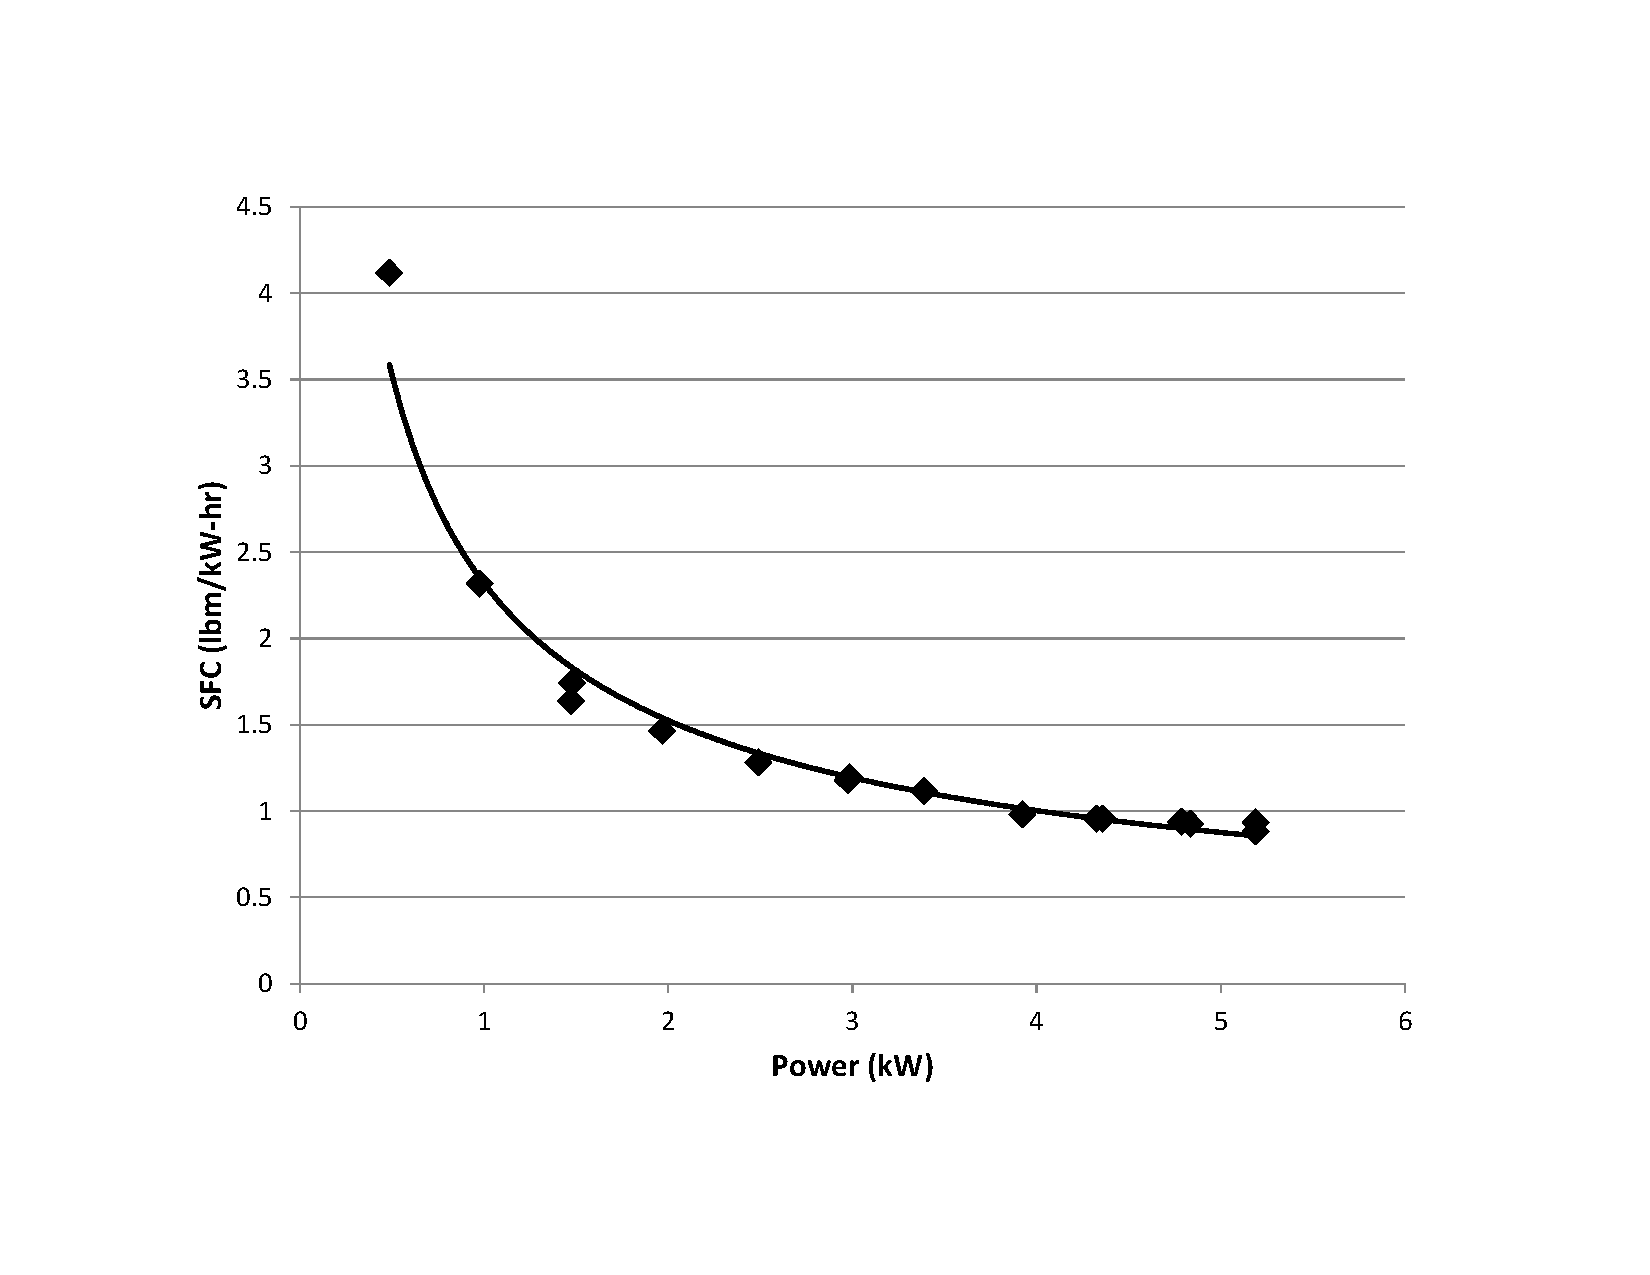
\includegraphics[width=5in]{SFC_plot.pdf} 
   \caption{Experiment SFC fitted with power-law regression}
   \label{fig:example}
\end{figure}

% Figure 5 - Thermal Efficiency vs Power
\begin{figure}[h!] %  figure placement: here, top, bottom, or page
   \centering
   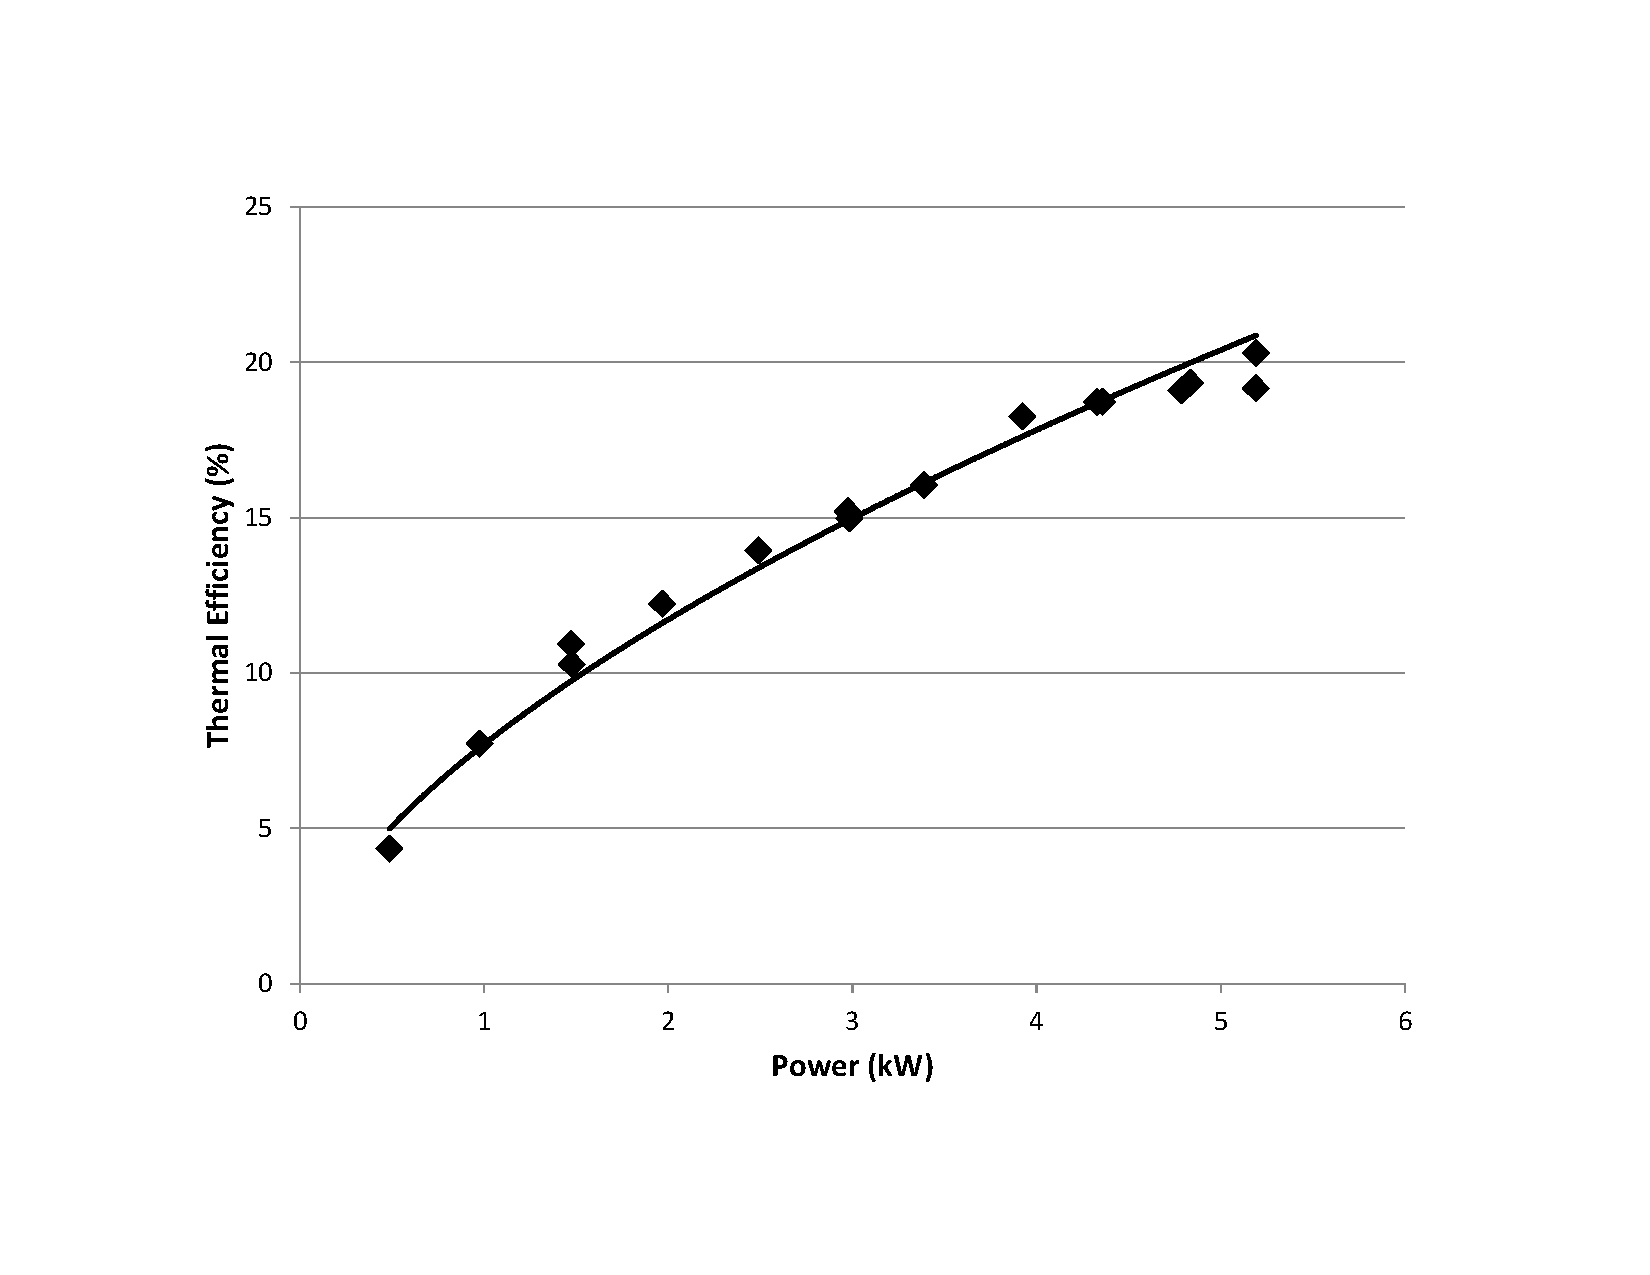
\includegraphics[width=4.5in]{thermal_efficiency_plot.pdf} 
   \caption{Experiment thermal efficiency fitted with power-law regression}
   \label{fig:example}
\end{figure}


\begin{equation}
SFC = 2.3175P^{-0.604}
\end{equation}

\begin{equation}
\eta_{th} = 7.7085P^{0.6045}
\end{equation}


\newpage

\section*{\fontsize{12}{12}\selectfont DISCUSSION}
It can be seen graphically in Figure 4 that the SFC regression matches the data well. The correlation coefficient, calculated to be $r_{SFC} = 0.99$, gives confidence that the regression model is sufficiently accurate for modeling the performance of the generator with this system. The same can be said for the thermal efficiency regression shown in Figure 5. The correlation coefficient for thermal efficiency $r_{th} = 0.99$ gives high confidence that this regression is also sufficiently accurate to use for modeling the system.\bigskip

The trend shown in Figure 4 makes logical sense because the mass rate does not change much from experiment to experiment, so an increase in power supplied to the resistance heaters would decrease the SFC according to Equation (1). The trend shown in Figure 5 for thermal efficiency also makes sense, as according to Equation (2) it is technically the inverse of the SFC divided by a constant (Lower Heating Value, LHV).

\section*{\fontsize{12}{12}\selectfont CONCLUSION}

\begin{itemize}

\item An experiment has been conducted to observe the performance of a Honda EM5000SX Engine-Generator.

\item The SFC and thermal efficiency of the engine-generator system were calculated for each run of the experiment, and are plotted along with regression models in Figure 4 and Figure 5.

\item The regression models calculated for both SFC and thermal efficiency are shown to accurately model the system, with correlation coefficients calculated to be $r_{SFC} = 0.99$ and $r_{th} = 0.99$.

\item The behavior for SFC and thermal efficiency observed in the experiment matches that of other small engine-generator systems as shown in Figure 1 and Figure 2 \cite{Silva}.

\end{itemize}



\section*{\fontsize{12}{12}\selectfont REFERENCES}

\begin{thebibliography}{2}

\bibitem{Silva}
Silva, Marcelo Jose Da et al., 2013, "Comparative Analysis of Engine Generator Performance Using Diesel Oil and Biodiesels Available in Parana State, Brazil," \emph{Renewable and Sustainable Energy Reviews}, vol. 17, pp. 278-82
\end{thebibliography}




\end{document}
----------------------------%TEmplates-------------------------------

-------------------------Figure-----------------------

\begin{figure}[h!]  
  \centering
    \includegraphics[width=\linewidth]{**file**}
    \caption{Docking Station}
\end{figure}

---------------------------Table-----------------------
\begin{table}[ht]
\caption{Nonlinear Model Results} % title of Table
\centering % used for centering table
\begin{tabular}{c c c c} % centered columns (4 columns)
\hline\hline %inserts double horizontal lines
Case & Method\#1 & Method\#2 & Method\#3 \\ [0.5ex] % inserts table
%heading
\hline % inserts single horizontal line
1 & 50 & 837 & 970 \\ % inserting body of the table
2 & 47 & 877 & 230 \\
3 & 31 & 25 & 415 \\
4 & 35 & 144 & 2356 \\
5 & 45 & 300 & 556 \\ [1ex] % [1ex] adds vertical space
\hline %inserts single line
\end{tabular}
\label{table:nonlin} % is used to refer this table in the text
\end{table}



probably best to insert as an image from excel

\bigskip\\
\begin{table}[h!]
  \caption{}
  \includegraphics[width=\linewidth]{**file**}
\end{table}
\bigskip\\





-----------------------------Equations------------------------
-----------------------------Regular
\begin{equation}
a = b + c
\end{equation}

--------------------------------- Multiline
\begin{multline}
a = b + c + d + e + f
+ g + h + i + j \\
+ k + l + m + n + o
\end{multline}

-------------------------------Citations-------------------------
\bibitem{Author last name}
  Last, First., year of publication,
  article name, book(etc) name, from \\
  link goes here

----------------------------------other-----------------------------

equations:
http://moser-isi.ethz.ch/docs/typeset_equations.pdf

citations:
http://library.missouri.edu/engineering/about/guides/asme
https://www.asme.org/shop/proceedings/conference-publications/references